% ---------- Datei: chapters/05_test_und_qa.tex ----------
\chapter{Test- und Qualitätssicherung}

\section{Testkonzept}
Die Testphase fokussiert sich auf die zentralen Projektziele: Erreichbarkeit, Routing und Failover. Für die Tests wurden temporär öffentliche IP-Adressen und eine SSH-Regel konfiguriert, da der Zugriff über IAP (Identity-Aware Proxy) im isolierten Ausbildungsprojekt nicht vollständig zur Verfügung stand. Der eigentliche Testverkehr wurde dabei strikt über die internen IP-Adressen \texttt{10.10.x.x} und \texttt{192.168.x.x} geroutet.

\section{Durchführung}
Die Tests wurden direkt nach dem Deployment durchgeführt. Der Ping-Test war erfolgreich. Die Verbindung zwischen den Test-VMs war stabil und ohne Paketverlust.

Der Traceroute-Test wurde explizit mit ICMP ausgeführt, um den exakten Routing-Pfad über das VPN abzubilden (da Standard-UDP-Traffic von der Firewall blockiert wird). Die Ausgaben belegen, dass der Datenverkehr korrekt über die interne VPN-Verbindung geleitet wird.

\subsection{Routing}
Die Überprüfung der BGP-Routen erfolgte direkt im Cloud Router. Die Systemausgabe zeigt, dass die Präfixe korrekt gelernt wurden und beide Tunnel als aktiv angezeigt werden.

\begin{figure}[!ht]
\centering
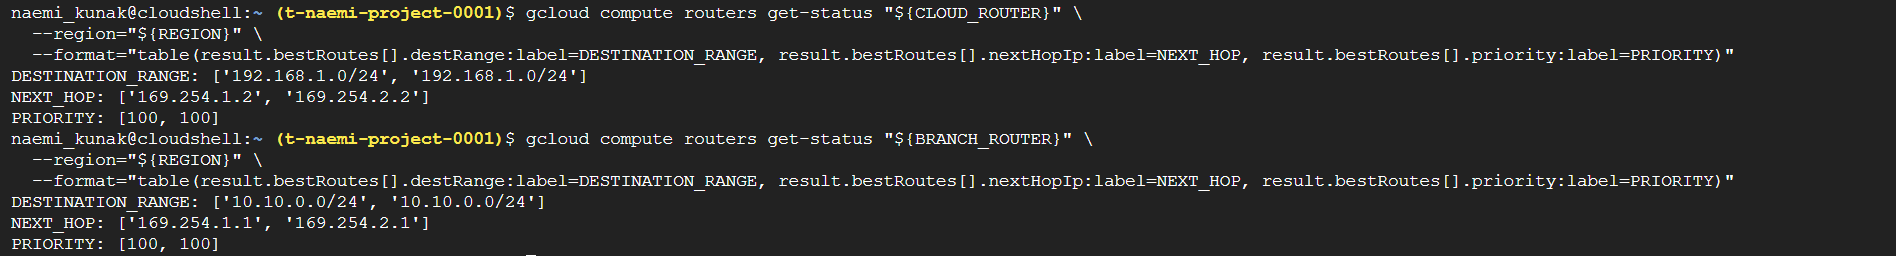
\includegraphics[width=\textwidth]{images/BGP-Routes.png}
\caption{BGP-Routen}
\end{figure}

\subsection{Firewall}
Die Firewall-Regeln wurden restriktiv konfiguriert, sodass nur der notwendige Testverkehr zugelassen war. Dies bestätigt die erfolgreiche Umsetzung des \textit{Default-Deny}-Prinzips.

\begin{figure}[!ht]
\centering
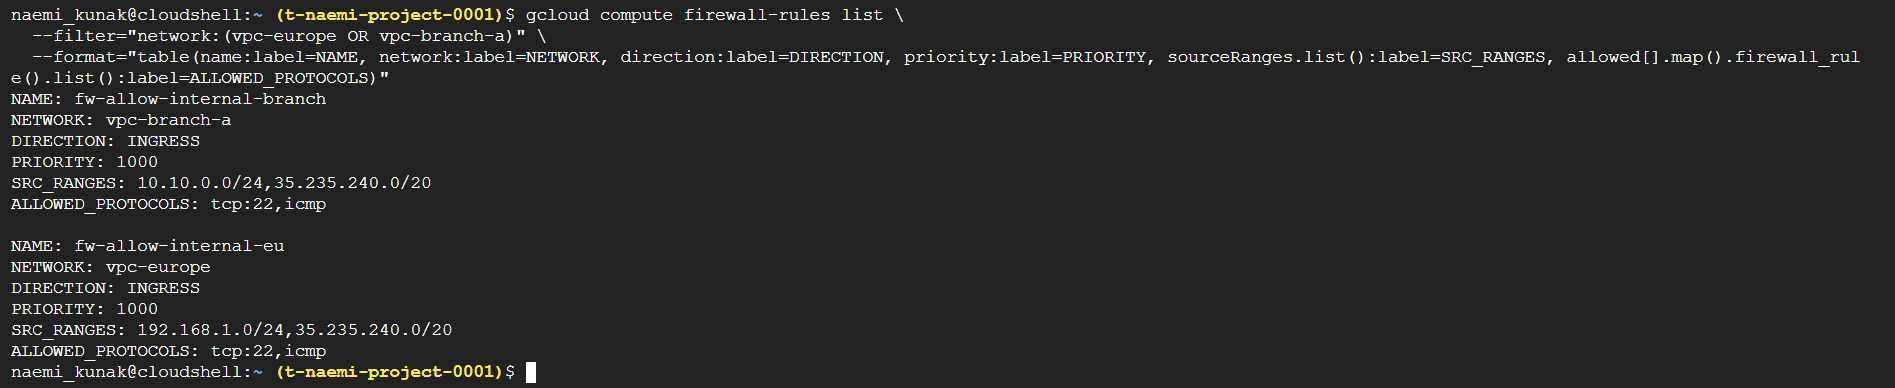
\includegraphics[width=\textwidth]{images/Firewall_rules.png}
\caption{Firewall-Regeln}
\end{figure}

\subsection{Failover}
Für den Failover-Test wurde die BGP-Sitzung von \textit{Tunnel 0} administrativ entfernt. Nach einer kurzen Konvergenzzeit lief der Datenverkehr automatisch über den redundanten \textit{Tunnel 1} weiter. Damit wurde die Redundanz der Verbindung erfolgreich nachgewiesen.

\begin{figure}[!ht]
\centering
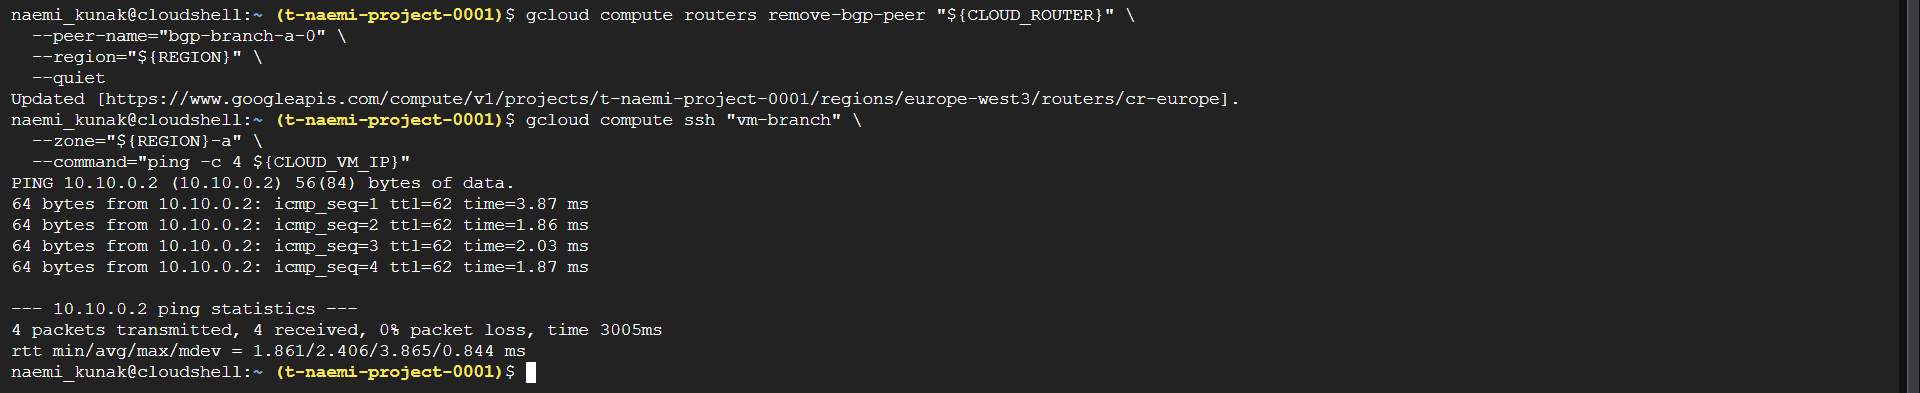
\includegraphics[width=\textwidth]{images/Failover.png}
\caption{Failover-Test}
\end{figure}


\section{Ergebnis}
Alle definierten Testfälle waren erfolgreich. Die Verbindung zwischen der Cloud und der On-Premises-Umgebung war stabil, das dynamische BGP-Routing funktionierte reibungslos und der automatische Failover auf den redundanten Tunnel wurde korrekt ausgeführt.